%settings

\setlength{\parindent}{2ex}
\phantomsection
%text
%--------------------------------------Task1----------------------------------
\section{Model of the project with Collaboration Diagrams.}
The Figure \thesection.1 shows communications in between an Admin online user and the interface \& database that happen in the Initialization form.
\begin{figure}[h!]
	\centering
	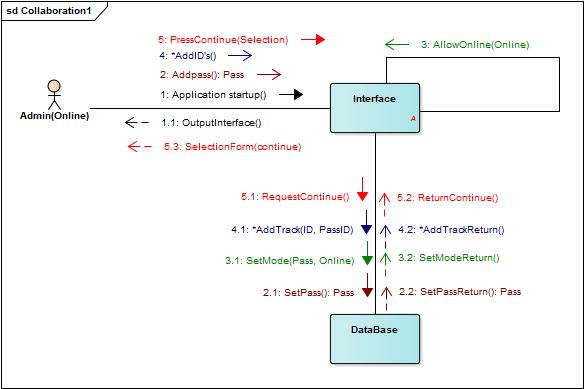
\includegraphics[keepaspectratio=true,scale=0.7]{Collaboration1}
	\caption{Initialization Form} 
\end{figure}
\begin{flushleft}
\begin{enumerate}
   \item[1] User initializes the application.
   \begin{itemize}
     \item[1.1] The application shows the interface to the user, showing its own ID.
   \end{itemize}
   \item[2] User inputs a password in order to go online.
   \begin{itemize}
     \item[2.1] The interface sends to the database the password.
     \item[2.2] Returns the control to the user.
   \end{itemize}
   \item[3] User can now go online, by checking the allow online checkbox in the interface.
   \begin{itemize}
     \item[3.1] The interface sends to the database the online mode initialization
     \item[3.2] The user can now proceed to become an admin.
   \end{itemize}
   \item[4] User inputs ID's of other users.
   \begin{itemize}
     \item[4.1]	The password and ID inputted in the interface registers the tracked person.
     \item[4.2] Returns control to user to input other local users to track.
   \end{itemize}
   \item[5] User presses continue to proceed to next form.
   \begin{itemize}
     \item[5.1] Interface requests the continue method from the database.
     \item[5.2] Database returns the continue method therefor continuing to Selection form
     \item[5.3] Selection form is outputted to user.
   \end{itemize}
\end{enumerate}
\end{flushleft}
The Figure \thesection.2 shows communications in Selection form that happen between an Admin online user, the interface that exchanges data with database which dictates the track method and other local user functions.
\begin{figure}[h!]
	\centering
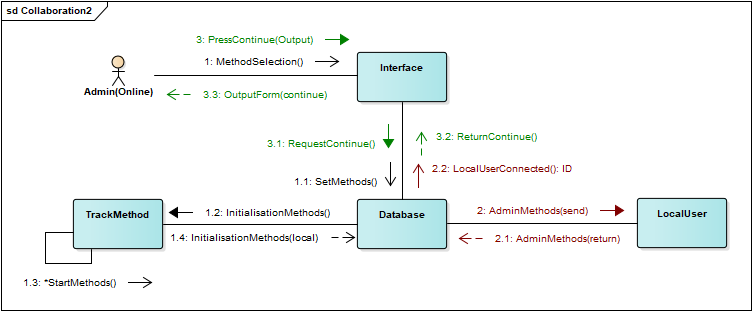
\includegraphics[keepaspectratio=true,width=\textwidth]{Collaboration2}
	\caption{Selection Form} 
\end{figure}
\begin{flushleft}
\begin{enumerate}
   \item[1] User selects the track methods he wants to use.
   \begin{itemize}
     \item[1.1] The interface Sets the methods in the database.
     \item[1.2] Database Requests initialization of the track methods
     \item[1.3] Each track method is started in the track method to start tracking data from other local users or the pc itself.
     \item[1.4] The track method component sends to the database that the local methods were initialized.
   \end{itemize}
   \item[2] The database sends the Methods to Local Users.
   \begin{itemize}
     \item[2.1] The database recives the id of the users that are currently present in the LAN. 
     \item[2.2] Interface shows which users are currently connected in LAN.
   \end{itemize}
   \item[3] User Presses button continue for the output form.
   \begin{itemize}
     \item[3.1] Interface requests from the database the output form.
     \item[3.2] Interface recieves the output form.
     \item[3.3]  User sees the output form.
   \end{itemize}
\end{enumerate}
\end{flushleft}
\begin{figure}[h!]
	\centering

The Figure \thesection.3 shows communications in Output form that happen between the same components as in Figure 1.2.	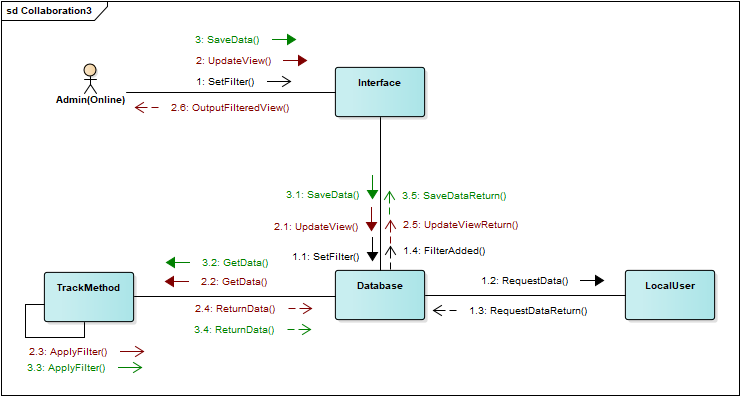
\includegraphics[keepaspectratio=true,width=\textwidth]{Collaboration3}
	\caption{Output Form} 
\end{figure}
\begin{flushleft}
\newpage
\begin{enumerate}
   \item[1] User types a filter for data in the iterface. 
   \begin{itemize}
     \item[1.1] Interface saves the filter into database.
     \item[1.2] The database requests filtered data from the local users.
     \item[1.3] Local users send the filtered data to the admin Database.
     \item[1.4] Interface recieves confirmation that the filter was added.
   \end{itemize}
   \item[2] User updates view to see the data collected.
   \begin{itemize}
     \item[2.1] Interface request for updated view.
     \item[2.2] Database requests data from tracking methods.
     \item[2.3] Track method component applies filter to the collected data.
     \item[2.4] Filtered data is returned to the database.
     \item[2.5] Update view outputs the collected filtered data.
     \item[2.6] User views the data.
   \end{itemize}
   \item[3] User presses button to save of data.
   \begin{itemize}
     \item[3.1] Interface requests data from the database. 
     \item[3.2] Database requests data from tracking methods.
     \item[3.3] Track method component applies filter to the collected data.
     \item[3.4] Filtered data is returned to the database.
     \item[3.5] The save file is made outputting a confirmation message on the interface.
   \end{itemize}
\end{enumerate}
\end{flushleft}
%-Task2----------------------------------
\section{Technologies planned on using in the project}
The technologies planned for using in this project are the following:
\begin{itemize}
\item \textbf{Operating system:} Windows,Linux,Mac OS,Android,Windows phone.
\item \textbf{Programming languages:} C,C++, Sql.
\item \textbf{IDEs:} Qt(Cross-platform framework).
\end{itemize}
\textbf{Qt} is a cross-platform application framework that is used for developing application software that can be run on various software and hardware platforms with little or no change in the underlying codebase, while still being a native application with native capabilities and speed.\par
Cross-Platform means that the application should work under all operating system.\par
As For programming languages C and C++ are the fastest compiling high level languages, and Sql is a system query language which helps with in working with the databases.
\clearpage